%chktex-file 36
%chktex-file 23
%chktex-file 10
%chktex-file 17
%chktex-file 9
\documentclass[computationalMathematics.tex]{subfiles}

\begin{document}

%%%%%%%%%%%%%%~~~~~~~~~~~~~~~~~~~~~~~~~~~~~~~~~~~~~~~~%%%%%%%%%%%%%%%
\section{19th of September 2018 --- A. Frangioni}
%%%%%%%%%%%%%%~~~~~~~~~~~~~~~~~~~~~~~~~~~~~~~~~~~~~~~~%%%%%%%%%%%%%%%

This course will deal with the optimization and numerical analysis of machine learning problems.
We are not going to solve difficult problems (e.g. NP-hard problems), besides we try to find an efficient solution for simple ones (often \textbf{convex} ones), since we are dealing with huge amount of data.

Let us start with a warm up on machine learning problems.

\subsection{Introduction to machine learning problems}

Machine learning techniques are not as ``young'' as it might seem, the intuition has been there for ages, but we did not have enough calculus power.
Machine learning algorithms are starting working well nowadays, thanks to the many improvements in computer performances; for this reason, it is becoming a more and more popular subject to study.

The main idea behind machine learning is to take a huge amount of data (e.g.~frames of a video for object-recognition) and squeeze them, in order to process them.
This intuitive concept is translated in mathematical terms as ``building a \textbf{model}'' that fits our data.
As in practical engineering problems, people want to construct a model (a small sized representation of the large thing we want to produce in the end) and try to understand its behaviour, before actually build the thing.
Take as an example the problem of designing a jet.
It is not clever to start building the plane before designing a cheap prototype to better study its behaviour in the athmosphere.

The kind of models we want to build are cheap to construct and as close as possible to the real problem we are studying.
In phisics, people try to find the best mathematical model to describe a real world phenomenon.
The main issue is computation, since the more accurate the model, the more costly the prediction phase.
Hence, a model is a good when it is a good tradeoff between accuracy and simplicity, namely it provides good prediction without incurring in slow computations.

The model, though, has to be parametric: we do not have only one model, we have a ``shape'' of a model, which is fit to our problem through the tuning of some parameters.

\begin{example}
  As an example, we are given three couples: $f(x_1) = y_1$, $f(x_2) = y_2$, $f(x_3) = y_3$, as shown in \Cref{fig:19sett1}.

  \addpic{0.6}{pics/19sett/1.png}{Geometic representation of the input. We are interested in finding a model that fits the input data and allows to predict $\bar{y}$ out of $\bar{x}$.}{fig:19sett1}

We need to make some choices: first, we need to decide the kind of model we believe is a good approximation of the objective function, say a linear model $f(x) = ax + b$.
  After doing that, we are left with choosing its parameters (in order to pick a line among the whole family of functions), namely $a$ and $b$.
\end{example}

The aim of machine learning is to build a model that fits the data we are given and then to tune parameters in order to achieve a good ``predicting power'' on unseen inputs (in machine learning the technical term is ``not \textbf{overfitting}'', see \Cref{overfitting}).

Another important characteristic of a good model is that it should not take too long to be built.

In this course we do not concentrate on the problem of finding the model that best fits our data, but we are already given a problem and a model and we only study its behaviour through its parameters.

\subsection{Optimization}

In the rest of this lecture we are going to understand what an optimization problem is, through some intuitive real world examples.

\subsubsection{Linear estimation}
\begin{definition}[Linear model]
  Let $f: \R^n \to \R^n$ be the objective function. We call $\widetilde{f}(x) = \sum_{i = 1}^n w_i x_i + w_0 = w x + w_0$ the \textbf{linear model} of $f$ for a given set of parameters, which is a vector $w = (w_0, w_1, \ldots, w_n) \in \R^{n+1}$.
\end{definition}

How can we evaluate the ``similarity'' between our model and the objective function? Through computing the ``error'' or difference between the objective function and the model on each input.
Under this assumption, the error function may be used to find the best parameters for our model, through a minimum problem:

\begin{definition}[Least squares problem]
  Let $f: \R^n \to \R^n$ be the objective function, such that $f(x) = y$ and let $Xw$ be our linear model. Then we can find the best values for vector $w \in \R^{n+1}$ by computing 
\[
  \min_{w} \norm{y - X w}
\]
\end{definition}

If the matrix $X$ is invertible then the simple solution is $w = \inv{X}y$.
The point is that this operation is very costly when dealing with a huge number of entries.

\subsubsection{Low-rank approximation}
We may want to approximate a matrix $M \in M(n, m, \R)$ as the product between two smaller matrices: $A\in M(n, k, \R)$ and a ``fat and large'' $B\in M(k, m, \R)$ ($k\ll n, m$).

\[
  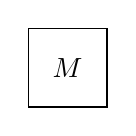
\begin{tikzpicture}[baseline=(current bounding box.center)]
    \draw (0,0) rectangle (1,1);
    \node at (0.5,0.5) {$M$};
  \end{tikzpicture}
  \approx
  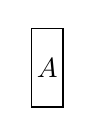
\begin{tikzpicture}[baseline=(current bounding box.center)]
    \draw (0,0) rectangle (0.4,1);
    \node at (0.2,0.5) {$A$};
  \end{tikzpicture}
  \cdot
  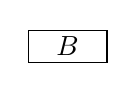
\begin{tikzpicture}[baseline=(current bounding box.center)]
    \draw (0,0) rectangle (1,0.4);
    \node at (0.5,0.2) {$B$};
  \end{tikzpicture}
\]

This problem can be translated into a numerical analysis problem of the following shape
\[
  \min_{A, B} \norm{M - AB}
\]


\subsubsection{Support vector machines}

Let us take a decision problem: given a set of values of many parameters (aka variables) ``label'' a person as ill or healthy.

The geometric intuition in two dimensions is given by \Cref{fig:19sett2}.
We would like to find the line that better splits the plane into two regions.
The rationale here is to maximize the space between the line and the nearest points (called \textbf{margin}), in order to have a better accuracy.

\addtwopics{0.4}{pics/19sett/svm4.pdf}{0.4}{pics/19sett/svm5.pdf}{There are many possile boundaries that can be chosen as a model using many angular coefficients. Our best guess is the one that maximizes the distance between the line and the nearest points.}{fig:19sett2}

The maximum-margin separating hyperplane is the solution of
\[
  {\min\limits_w \big\{\sqrnorm{w_+}~:~y^i( w_+ x^i + w_0 ) \geq 1, ~ i = 1, \ldots, m \big\}}
\]
       
where the margin is $\frac{2}{\norm{w_+}}$, assuming any exists.

In fact, what happens most of the times is that there is no such line. 
To overcome this issue we introduce the concept of ``penalty'' that accounts for the number of points that are misclassified.

\begin{definition}[Multi-objective optimization problem]
\[
  \textstyle \min\limits_{w,\xi} {\sqrnorm{w_+} + C \sum\limits_{i=1}^m \xi_i}
\]
where $y^i( w_+ x^i + w_0 ) \geq 1 - \xi_i, ~ \forall i = 1, \ldots, m$ and $xi_i \geq 0, ~ \forall i = 1, \ldots, m$, where $C$ is called \textbf{hyperparameter}.

This formula formalizes the intuition that the approximated function may have a greater norm and lead to a very small misclassification error, or it could be the other way round.
  Both these solutions are acceptable and their performances depend only on the problem.
\end{definition}

This whole course has the aim of presenting some techniques for solving efficiently \textbf{convex quadratic problems}, as the ones presented above.

Whenever we are able to solve the multiobjective optimization problem we are also able to solve what is called the \textbf{dual problem}, which is formally defined in \Cref{dual} and has the following shape in our case:

\[
  \max\limits_{\alpha} \Biggl \{ \sum\limits_{i=1}^m \alpha_i - \frac{1}{2} \sum\limits_{i=1}^m \sum_{j=1}^m \alpha_i \ps{x^i}{x^j} \alpha_j \Biggr \}
\]

where $\sum\limits_{i=1}^m y^i \alpha_i = 0$ and $0 \leq \alpha_i \leq C, ~ \forall i = 1, \ldots, m$.

\end{document}
